\customsection{Pruebas y resultados}

\subsection{Pruebas unitarias}
Las pruebas explicadas en este segmeto involucraron clases internas de los 3 grandes programas del proyecto: el backend, la User App, y el House Manager. Es decir, se probaron los componentes más simples del sistema como se muestra a continuación:

\begin{itemize}
	\item \textbf{House Manager:} Las pruebas unitarias explicadas a continuación involucraron paquetes de terceros y rutinas propias.
	\begin{itemize}
		\item El documento ``\_\_\_prueba spectrum.py'' contiene la prueba de renderizado de los paquestes de Python Pyqtgraph y Pyside juntos en una misma ventana.
		\item El archivo ``smtp\_test\_privateemail.py'' contiene la prueba para verificar el proceso de envio de e-mails utilizando el dominio ``alfagenos.com''.
		\item El documento ``test\_http\_request.py'' fue utilzado para realizar pruebas de conunicación a travez de solicitudes Https tipo post desde el lenguaje de programación de Python.
		\item El programa ``test\_mqtt.py'' prueba el componente de comunicación del House Manager que utiliza el protocolo de comunicación mqtts.
		\item El archivo ``test\_oauth.py'' prueba el servicio de autenticación de Google y el manejo de las credenciales; su creación y eliminación.
	\end{itemize}
	\item \textbf{User app:} Las pruebas unitarias de esta aplicación se realizaron renderizando objetos en una ventana de prueba desactivada para la version de lanzamiento. Los objetos probados fueron los contenidos en los archivos: ControlScreen.js, MeasureScreen.js, IntroScreen2.js, Timer.js, MyChart.js
	\item \textbf{Backend:} Las pruebas del backend se realizaron a los diferentes microservicios implementados. Los scripts de prueba fueron:
	\begin{itemize}
		\item El programa ``test\_control\_SENDER\_SUBSCRIBER.js'' se utilizo para probar el servicio de control del backend desde la perspectiva del generador y receptor de la orden.
		\item El archivo ``test\_measure\_SENDER\_SUBSCRIBER.js'' contiene la prueba para verificar el proceso de reporte de datos.
		\item El programa ``test\_get\_history.js'' fue utilzado para probar el servicio de solicitud de datos para cierto rango de tiempo.
		\item El archivo ``test\_send\_command.js'' prueba el servicio de envío de mensajes mqtts a dispositivos específicos a través de solicitudes Https tipo ``post''.
	\end{itemize}
\end{itemize}

\subsection{Pruebas de integración}

Para finalizar, debido a que el sistema desarrollado está constituido enteramente por software se decidió adicionar un componente de hardware para probar conceptualmente la capacidad de añadir cualquier sistema de medición o actuación.
\vspace{0.5cm}\\
Como dispositivo de medición se utilizó un medidor bifásico de la empresa Inelca con una interfaz de comunicación Rs485 \ref{fig_32}. Utilizando esta interfaz y un conversor USB a Rs485 se logró comunicar la Raspberry con el medidor de Inelca.
\vspace{0.5cm}\\
\begin{figure}[htbp]
	\centerline{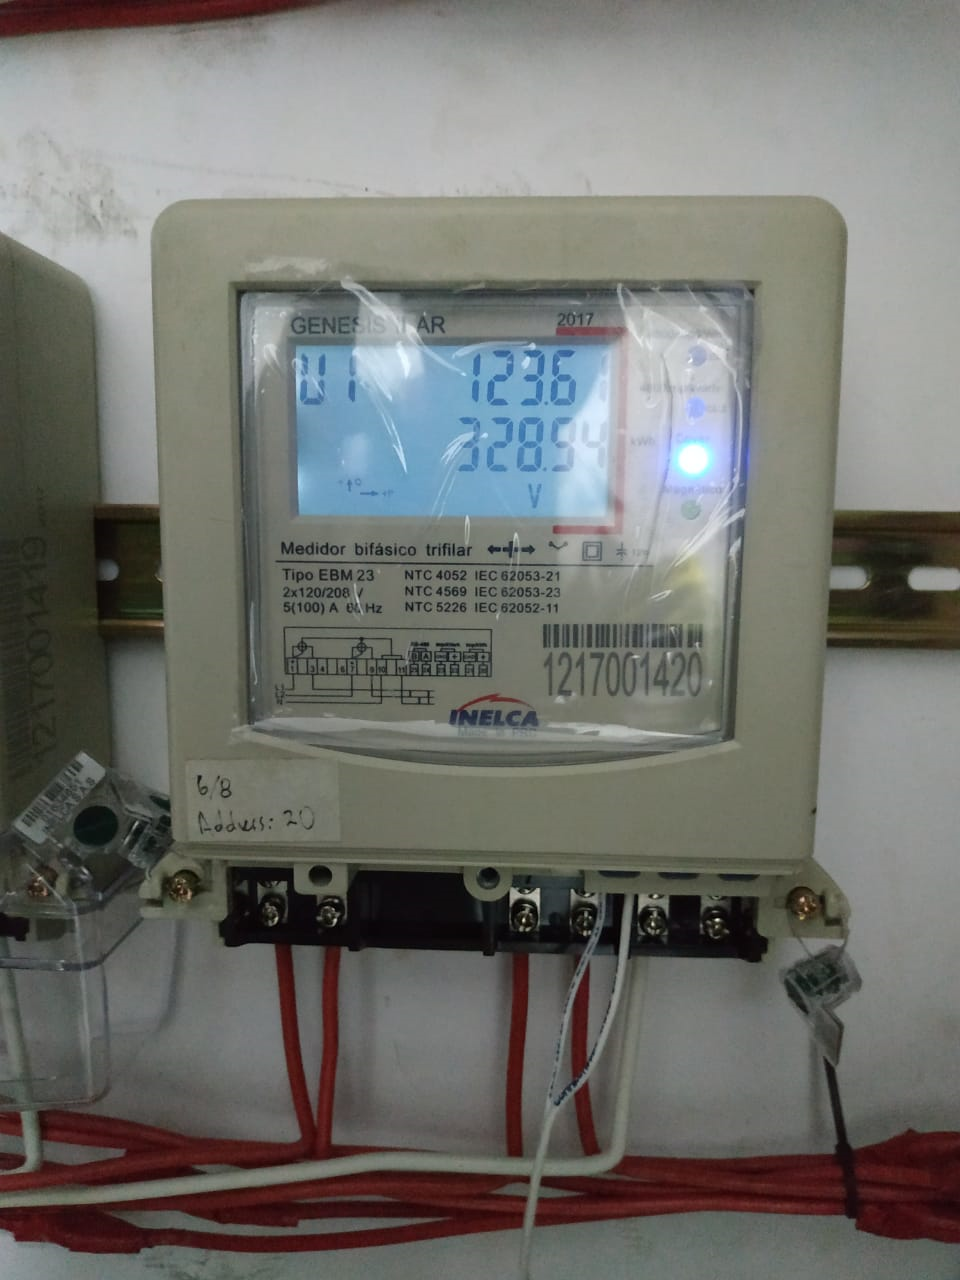
\includegraphics[width=9cm]{./figuras/concepto_1.png}}
	\caption{Dispositivo Inelca utilizado para la prueba de concepto. Fuente: propia}
	\label{fig_32}
\end{figure}

Para finalizar, se puso a prueba el sistema añadiendo la función de adquisición necesaria para obtener el valor del voltaje de valor cuadrático medio (Rms) de la linea U1 del medidor. La funcion utilizaba un rutina a partir del cual se generaban y se interpretaban las tramas para adquirir el valor de voltaje del medidor. Una foto de todos los sistemas funcionando en conjunto se observa en la figura \ref{fig_33}.

\begin{figure}[htbp]
	\centerline{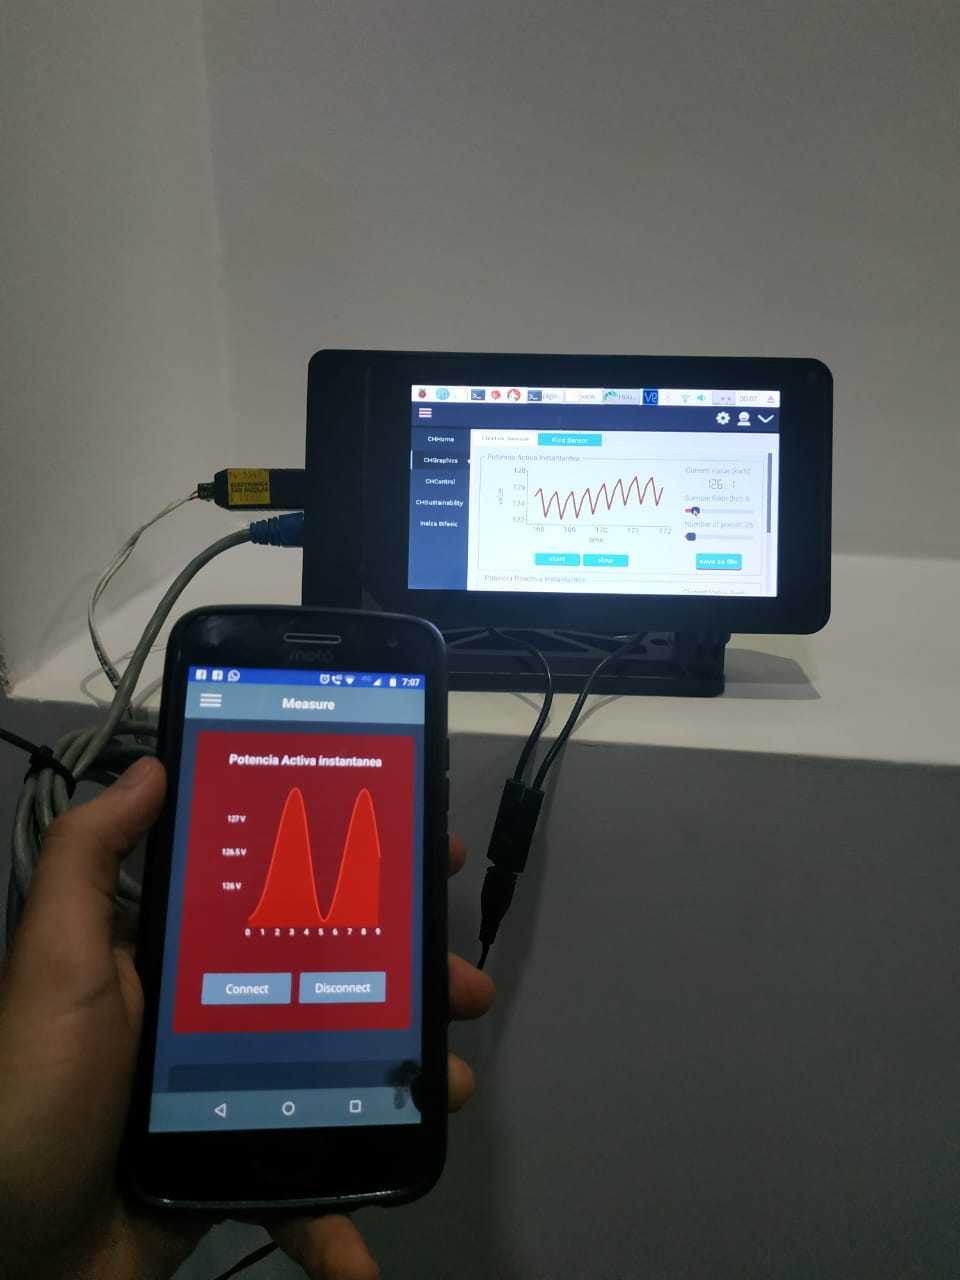
\includegraphics[width=10cm]{./figuras/concepto_2.png}}
	\caption{Prueba de concepto usando todos los sistemas. Fuente: propia}
	\label{fig_33}
\end{figure}

\subsection{Resultados}
A lo largo de este proyecto de grado, se construyó un sistema de administración de datos ``serverless'' para sensores y actuadores. Para ello se utilizaron los protocolos de comunicación Https y Mqtts y los servicios de almacenamiento SQL y Google Cloud Storage. La selección de estas herramientas le permitió al sistema monitorear y controlar los sensores y actuadores, conectados al sistema desde la Raspberry, de manera local y remota. La estructura en la cual se implementó el proyecto permitió que contara con las siguientes características:
\begin{itemize}
	\item Los tiempos de respuesta del backend fueron en promedio de 1.31 segundos para el proceso mas demorado del sistema: reportar un dato, almacenarlo y enviarlo al dispositivo necesario usando Mqtts. Lo anterior teniendo en cuenta que el servidor de Google utilizado se encuentra en San Francisco USA.
	\item Las interfaces gráficas de ambos clientes (Escritorio y móvil) tienen el mismo estilo de diseño y son multiplataforma. Por una parte la aplicación de escritorio puede funcionar en Windows y Linux, por otra parte la aplicación móvil puede funcionar para Android y Ios.
	\item La estructura utilizada y la manera en la que se modeló el sistema hacen que éste sea escalable, es decir, posee la capacidad de expandirse en cuanto a numero de dispositivos y usuarios. En teoría, el sistema puede soportar 4000 dispositivos conectados al mismo tiempo y una cantidad de usuarios limitada por el espacio de memoria comprado para los servicios SQL y Google Cloud Storage.
	\item El sistema fue diseñado teniendo en cuenta dos niveles de cifrado: el primer nivel consta de la encriptación manejada directamente por el proveedor de servicios (Google) y el segundo consta del cifrado de las credenciales de los dispositivos utilizando el método RSA-256. En adición, respecto a la seguridad de los datos personales del usuario como numero celular correo, etc, el servicio de Google se encarga directamente de hacer la encriptación y almacenamiento de los mismos.
	\item La selección del proveedor de servicios (Google) le permitió al sistema estar protegido de ataques de denegación de servicio de nivel 4 o inferior como: inundaciones SYN, inundaciones de fragmentos de IP, agotamiento de puertos, entre otros.
	
\end{itemize}
Teniendo en cuenta el proceso de implementación y los resultados obtenidos, el sistema cumplió en un 81 por ciento los requerimientos funcionales esperados. Los requerimientos que no fueron satisfechos fueron el 1.3 y 1.7. El primero no fue implementado directamente en la aplicación móvil pero, a pesar de que no era un requerimiento como tal, se implemento en la aplicación de escritorio. El segundo no fue implementado en ninguna de las dos aplicaciones.
\vspace{0.5cm}\\
Dentro de la carpeta del proyecto del ``House Manager'' se pueden encontrar scripts que fueron importantes para el despliegue de la aplicación. Por ejemplo; en el directorio ``./src/installing/'' se encuentran los ejecutables para la instalación de la aplicación en Windows y Debian; en el directorio ``./src/test/'' se encuentran las rutinas de “testing” utilizadas para algunos scripts y objetos utilizados en el programa.
\vspace{0.5cm}\\
Adicionalmente, en la carpeta del proyecto del \textit{backend} se pueden encontrar los scripts de prueba de cada una de las funciones de nube. Por ejemplo; en el directorio ``./src/CLOUD\_device\_control/'' se encuentran la prueba unitaria con el nombre ``test\_control\_SENDER\_SUBSCRIBER.js'' de la función contenida en la carpeta. En cada una de las carpetas de cada función de nube se encuentra su respectiva prueba unitaria.
\vspace{0.5cm}\\
Finalmente, en la carpeta del proyecto del \textit{User App} se puede encontrar en el directorio raiz las ventanas de prueba: ``test\_App.js'' y test\_App2.js que fueron utilizadas para probar los componentes ubicados en el directorio ``./src/components/''. No todos los componentes de esta carpeta fueron utilizados en la aplicación final, puesto que no pasaban las de renderizado; esto se debe a que eran componentes basados en librerías abandonadas o dañadas.